\documentclass[11pt,a4paper]{article}
\usepackage[T1]{fontenc}
\usepackage[utf8]{inputenc}
\usepackage[french]{babel}
\usepackage{lmodern}
\usepackage{amsmath,amssymb}
\usepackage[margin=2.35cm]{geometry}
\usepackage{booktabs,longtable,tabularx}
\usepackage{enumitem}
\usepackage{graphicx}
\usepackage{xcolor}
\usepackage{microtype}
\usepackage{hyperref}

\hypersetup{colorlinks=true,linkcolor=blue!45!black,urlcolor=blue!45!black}
\setlist{nosep}
\newcommand{\code}[1]{\texttt{#1}}
\newcommand{\Kaut}{K^{*}_{\mathrm{aut}}}
\graphicspath{{../figures/}}

\title{Campagne M4.2 --- rapport préliminaire\\
\large effet de l'exposant de concavité $\gamma$ sur la statistique des
avalanches : exploration et confirmation}
\author{Programme M4.2 --- dossier \code{m4\_2\_credit\_soc}}
\date{27 juillet 2026}

\begin{document}
\maketitle

\begin{abstract}
Ce rapport préliminaire présente les résultats de la campagne M4.2 en
séparant strictement l'\textbf{exploration} (graines 1--3, volets 0--3,
5, 6) de la \textbf{confirmation} (graines disjointes 11--15, volet 4,
critères pré-enregistrés du protocole v1.1). \textbf{Résultat central} :
$\gamma$ déplace mesurablement $\hat\tau$ à $A=1$
($\Delta\hat\tau=-0{,}125$, IC95 $[-0{,}135;-0{,}115]$ pour
$\gamma=1/3$ contre le centre $\gamma=1/2$, persistant en taille, stable
aux fenêtres et à l'horizon doublé) --- le verdict machine du protocole
sur ce contraste est \textbf{PARTIEL} (6 des 8 conditions passent), non
CONFIRMÉ au sens strict, précisément parce que le contrôle d'échelle
apparié (condition 8), exécuté sur les mêmes graines confirmatoires,
montre que l'effet est \textbf{dominé par le déplacement du point fixe
autarcique} $K^*_{\mathrm{aut}}(\gamma)$ et non par la concavité en tant
que telle : à échelle égalisée, l'effet résiduel est petit et de
\textbf{signe opposé} ($+0{,}031$, IC95 $[+0{,}001;+0{,}061]$, marginal).
On démontre une invariance d'échelle exacte de la dynamique discrète qui
implique qu'à $\gamma$ fixé, $\hat\tau$ ne peut dépendre de $A,K_0$ qu'à
travers $K_0/K^*_{\mathrm{aut}}(\gamma,A)$ ; un test ciblé de cette
hypothèse corrobore sa partie nécessaire mais ne tranche pas, à la
précision disponible (3 graines), l'ampleur du résidu propre de
courbure. Le rapport de branchement reste épinglé institutionnellement
($b\in[0{,}30;0{,}32]$) et le canal de liquidité est quasi silencieux
(17 événements sur 102 runs distincts, exclusivement à $\gamma\ge2/3$).
Le modèle, la parité M4B et le protocole sont documentés dans
\code{spec\_m4\_2.pdf} et \code{protocole.pdf}.
\end{abstract}

\tableofcontents

\section{Cadre, modèle et vérifications préalables}

M4.2 généralise M4B (production $F_\gamma(K)=A K^\gamma$, taux dérivés des
rendements marginaux par moyenne géométrique, $k\equiv2$,
$\eta(N)=N$) ; définitions complètes dans \code{spec\_m4\_2.pdf}. Avant
toute campagne :
\begin{itemize}
\item 18 tests moteur (points 1--13 du cahier des charges), 2 tests de
parité, 8 tests d'estimateurs sur données synthétiques : tous verts ;
\item parité $\gamma=1/2$ contre M4B à $k=2$ : discret identique pas à
pas, écart flottant $\le3\cdot10^{-12}$ sur 1000 pas (spec §8) ;
\item trois audits indépendants en contexte frais (fidélité au cahier des
charges, invariants comptables, dérivation mathématique) : aucun bug ;
corrections documentaires intégrées ;
\item protocole pré-enregistré v1.1 figé avant le volet 1, intégrant
l'audit statistique indépendant (critères chiffrés, convention de coupure
hors portée, bootstrap obligatoire en confirmation).
\end{itemize}

Tous les runs de campagne sont des runs Simulation Lab étiquetés
\og M4.2 --- \code{<plan>} --- \code{<cellule>} \fg{} (décision
utilisateur) ; traçabilité complète en annexe et dans
\code{manifests/}. Configuration centrale : $\lambda=30$, $\delta=0{,}05$,
$\sigma=0{,}25$, $K_0=25$, $A=1$, fenêtre d'analyse $[T/4,T]$, fits par
graine puis agrégation (jamais de pooling).

\section{Volets exécutés}

\begin{center}
\begin{tabular}{llrl}
\toprule
Volet & Cellules & Runs & Statut\\
\midrule
0 benchmark & $\gamma\in\{1/3,2/3\}$ & 2 & ok (291\,s / 166\,s par run)\\
1 pilotes & 5 $\gamma$ $\times$ 3 graines $+$ sonde $0{,}75$ & 16 & ok, tous GO\\
2 taille finie & 5 $\gamma\times\lambda\in\{10,30,100\}$ & 45 & ok\\
3 horizon & 3 $\gamma$, $T=8000$ & 9 & ok\\
4 confirmation & $\gamma\in\{1/3,1/2,0{,}6,2/3\}$, graines 11--15 & 20 & \S\ref{sec:confirm}\\
5 ablation $A_{\mathrm{norm}}$ & $\gamma\in\{1/3,0{,}6,2/3\}$ & 9 & \S\ref{sec:ablation}\\
6 mécanisme & 5 $\gamma$, instantanés denses & 5 & \S\ref{sec:mecanisme}\\
\bottomrule
\end{tabular}
\end{center}
{\footnotesize Les 15 runs $\lambda=30$ du volet 2 sont les cellules
pilotes, réutilisées par identifiant déterministe (aucun recalcul).}

Aucune extinction, aucune censure par \code{pop\_max}, stationnarité
vérifiée sur toutes les cellules (critères pré-enregistrés : dérive
relative $\le4\,\%$, demi-fenêtres cohérentes en population et en
capital). Identifiabilité massive : 8\,300 à 34\,000 avalanches de taille
$s\ge2$ par run (seuil : 100).

\section{Exploration (graines 1--3) : la relation $\hat\tau(\gamma)$}
\label{sec:exploration}

\subsection{Fait central : dépendance non monotone}

\begin{center}
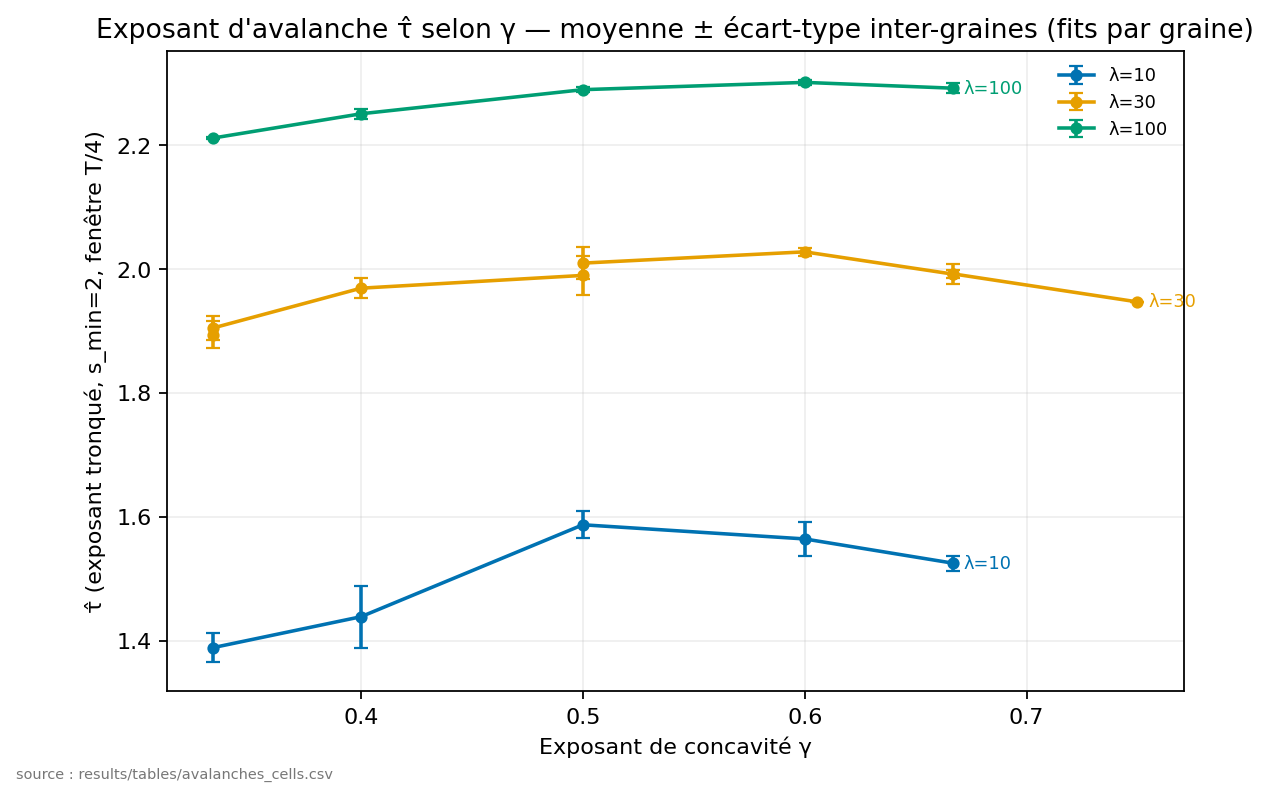
\includegraphics[width=.72\textwidth]{tau_vs_gamma.png}
\end{center}

Sur la fenêtre par défaut, métrique primaire $\hat\tau$ (exposant de la
loi tronquée, $s_{\min}=2$ ; à $\lambda=100$ la coupure est hors portée
pour toutes les graines --- drapeau pré-enregistré --- et $\hat\tau$ est
lu sur la loi pure) :

\begin{center}
\begin{tabular}{lccccc}
\toprule
$\hat\tau$ (moy.\ $\pm$ sd inter-graines) & $\gamma=1/3$ & $0{,}4$ & $1/2$ & $0{,}6$ & $2/3$\\
\midrule
$\lambda=10$ ($T{=}8000$) & $1{,}389\pm0{,}024$ & $1{,}439\pm0{,}050$ & $1{,}587\pm0{,}022$ & $1{,}564\pm0{,}028$ & $1{,}525\pm0{,}012$\\
$\lambda=30$ ($T{=}4000$) & $1{,}894\pm0{,}022$ & $1{,}969\pm0{,}016$ & $1{,}990\pm0{,}032$ & $2{,}028\pm0{,}007$ & $1{,}992\pm0{,}016$\\
$\lambda=100$ ($T{=}4000$, pur) & $2{,}212\pm0{,}002$ & $2{,}251\pm0{,}008$ & $2{,}290\pm0{,}004$ & $2{,}302\pm0{,}004$ & $2{,}292\pm0{,}008$\\
\bottomrule
\end{tabular}
\end{center}
Source : \code{results/tables/avalanches\_cells.csv}. Sonde exploratoire
$\gamma=0{,}75$ ($\lambda=30$, 1 graine) : $1{,}947$ — le repli continue.

Trois faits :
\begin{enumerate}
\item \textbf{les queues s'alourdissent à faible concavité} : le
contraste $\gamma=1/3$ vs $1/2$ vaut $-0{,}198$ ($\lambda=10$),
$-0{,}096$ ($\lambda=30$), $-0{,}078$ ($\lambda=100$) — même signe aux
trois tailles, amplitude $\ge\tfrac12$ de celle de $\lambda=30$ ;
\item \textbf{la relation est non monotone} : maximum vers
$\gamma\approx0{,}5$--$0{,}6$ puis repli, reproduit aux trois tailles ;
le contraste $\gamma=2/3$ vs $1/2$ est nul à $\lambda\ge30$
($+0{,}002$) ;
\item \textbf{robustesse} : fenêtres $T/8$--$T/2$ : variations
$\le0{,}005$ (fenêtres emboîtées — contrôle faible) ; horizon doublé
($T=8000$, $\lambda=30$) : contraste principal $-0{,}105$ vs $-0{,}096$.
\end{enumerate}

\subsection{L'artefact démographique jouerait en sens inverse}

$N/\lambda$ décroît fortement en $\gamma$ (de $22{,}0$ à $9{,}2$ sur la
grille, figure \code{demography\_vs\_gamma.png}) : à $\lambda$ fixé, les
cellules comparées n'ont pas la même population. Mais à $\gamma$ fixé,
$\hat\tau$ \emph{croît} avec la taille du système ($1{,}587$ / $1{,}990$
/ $2{,}290$ pour $\gamma=1/2$) : un pur effet de taille pousserait
$\hat\tau(\gamma{=}1/3)$ — population \emph{plus grande} — vers le haut.
On observe l'inverse : le confound démographique va contre l'effet
mesuré, qui est donc au pire sous-estimé. (Inférence, corroborée par la
persistance du contraste aux trois $\lambda$.)

\subsection{Coupure, branchement, scalings : la classe M4B est préservée}

\begin{center}
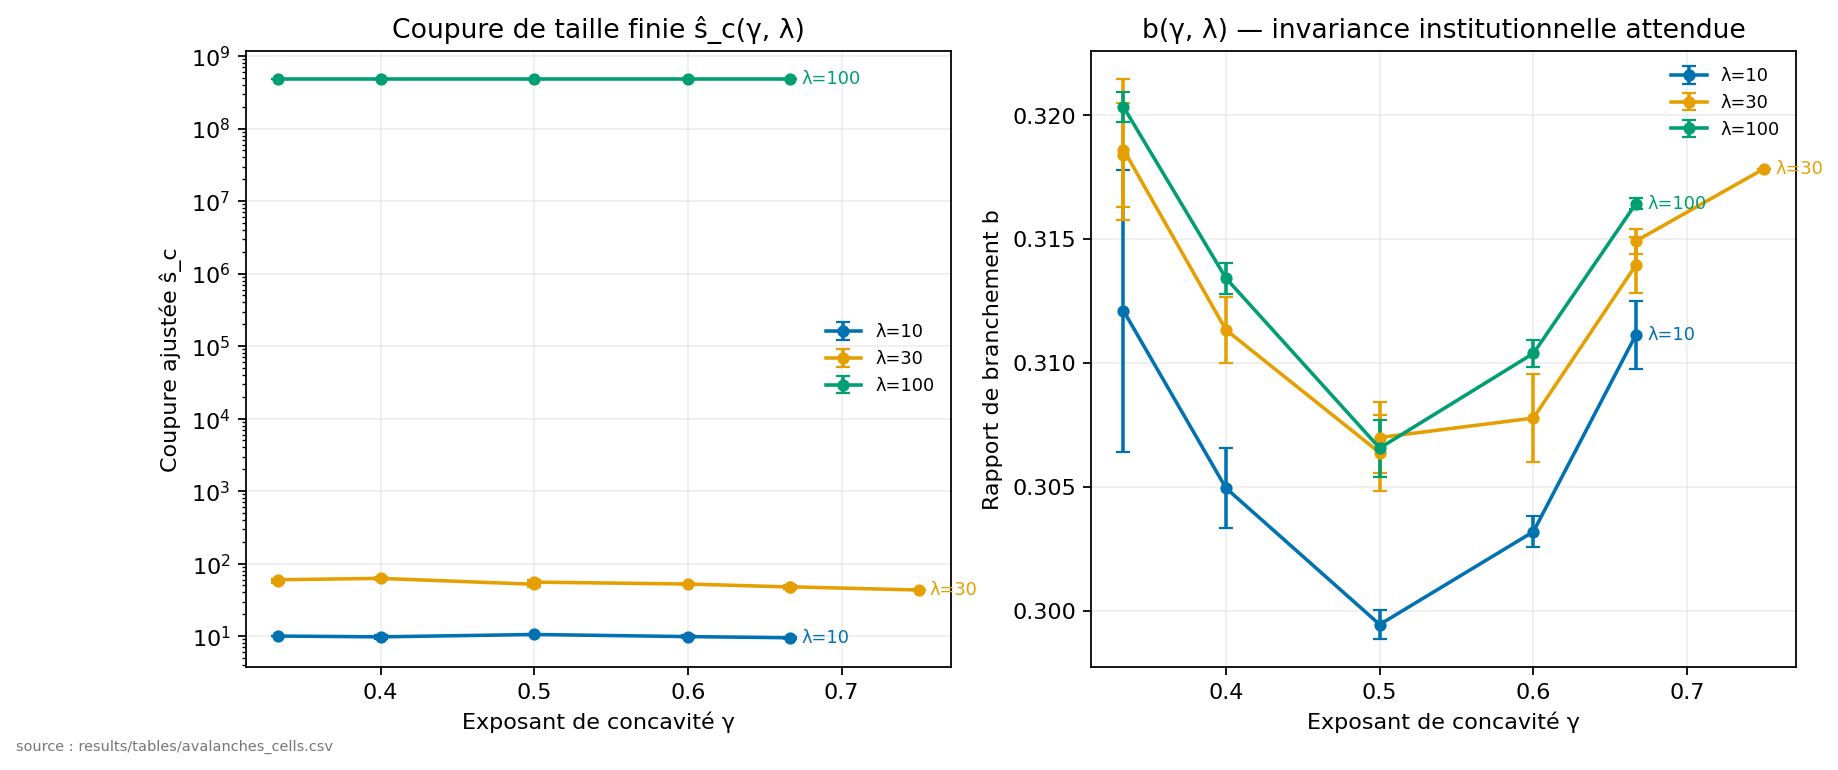
\includegraphics[width=.98\textwidth]{cutoff_branching_vs_gamma.png}
\end{center}

\begin{itemize}
\item \textbf{Coupure} : $\hat s_c\approx10$ à $\lambda=10$, $48$--$63$ à
$\lambda=30$ (variation modérée en $\gamma$, non monotone), hors portée
$3/3$ graines à $\lambda=100$ (comme dans la campagne M4B à $\lambda=100$
où elle sortait de la fenêtre). L'effet de $\gamma$ sur $\hat\tau$ ne se
réduit pas à un déplacement de coupure : à $\lambda=100$, la coupure est
hors portée \emph{dans toutes les cellules} et le contraste persiste sur
l'exposant pur.
\item \textbf{Branchement} : $b\in[0{,}299;0{,}320]$ sur les 19 cellules
— le plateau institutionnel $b\approx0{,}30$ (un round de marché par
tête) résiste à $\gamma$ \emph{et} à $\lambda$. Structure fine
reproductible : $b(\gamma)$ dessine un V peu profond, minimum à
$\gamma=1/2$, aux trois tailles — image miroir du maximum de
$\hat\tau$ ; piste mécanique prioritaire (\S\ref{sec:mecanisme}).
\item \textbf{Scalings} (figure \code{scaling\_lambda.png}, coupures
dégénérées exclues) : $\hat s_c\propto\lambda^{1{,}5-1{,}7}$ (2 points,
$10\to30$ ; M4B : $1{,}5$), $s_{\max}\propto\lambda^{0{,}55-0{,}62}$
(M4B : $0{,}58$), $\chi\propto\lambda^{0{,}52-0{,}61}$ (M4B : $0{,}51$),
l'exposant de $\chi$ étant légèrement plus fort à petit $\gamma$ —
cohérent avec des queues plus lourdes.
\end{itemize}

\subsection{Chaîne causale mesurée ($\lambda=30$)}
\label{sec:mecanisme-explo}

Source : \code{results/tables/observables\_cells.csv}.
\begin{center}
\begin{tabular}{lcccccc}
\toprule
& $\gamma{=}1/3$ & $0{,}4$ & $1/2$ & $0{,}6$ & $2/3$ & $0{,}75$\\
\midrule
taux médian du carnet & $0{,}024$ & $0{,}031$ & $0{,}049$ & $0{,}071$ & $0{,}094$ & $0{,}130$\\
prédiction $\gamma\delta/(1{-}\delta)$ & $0{,}018$ & $0{,}021$ & $0{,}026$ & $0{,}032$ & $0{,}035$ & $0{,}039$\\
intérêts / production & $0{,}45$ & $0{,}54$ & $0{,}67$ & $0{,}74$ & $0{,}76$ & $0{,}77$\\
âge moyen au décès (pas) & $22{,}0$ & $19{,}5$ & $15{,}4$ & $11{,}5$ & $9{,}2$ & $6{,}8$\\
contrats par tête & $10{,}7$ & $10{,}2$ & $8{,}9$ & $7{,}2$ & $5{,}8$ & $4{,}2$\\
levier $\Sigma D/\Sigma K$ & $1{,}38$ & $1{,}39$ & $1{,}30$ & $1{,}16$ & $1{,}09$ & $0{,}98$\\
morts par liquidité & $0\,\%$ & $0\,\%$ & $0\,\%$ & $0\,\%$ & $0\,\%$ & $0\,\%$\\
\bottomrule
\end{tabular}
\end{center}

Lecture (faits observés) : $\gamma$ élève les taux contractuels (de
$1{,}4$ à $2{,}7\times$ la prédiction autarcique, croissant avec
$\gamma$ : les contrats se signent entre entités bien sous
$K^*_{\mathrm{aut}}$, donc à rendements marginaux élevés), alourdit le
service relatif, raccourcit les vies, amincit le réseau (moins de
contrats par tête, levier plus faible). Le canal de liquidité est
\textbf{quasi silencieux mais pas rigoureusement nul} : $17$ défauts de
service distincts sur $102$ runs, \textbf{exclusivement à
$\gamma\ge2/3$} (jamais à $\gamma\le0{,}6$, jamais en confirmation) — un
signal physique cohérent avec l'alourdissement du service, pas un
artefact. La propagation reste très majoritairement une contagion de
bilan pure, et le levier de $\gamma$ opère surtout par la redistribution
des flux d'intérêts et la structure du réseau.

\section{Confirmation (graines 11--15)}
\label{sec:confirm}

Quatre contrastes confirmatoires (20 runs, 5 graines disjointes
$\{11,\dots,15\}$ chacun) : $\gamma\in\{1/3,0{,}6,2/3\}$ contre le centre
$\gamma=1/2$, évalués contre les 8 conditions pré-enregistrées du
protocole v1.1 (\code{scripts/analyze\_confirm.py},
\code{results/tables/confirm\_contrasts.csv}). Extraction avec bootstrap
obligatoire (condition 7) effectuée avant tout calcul de verdict.

\begin{center}
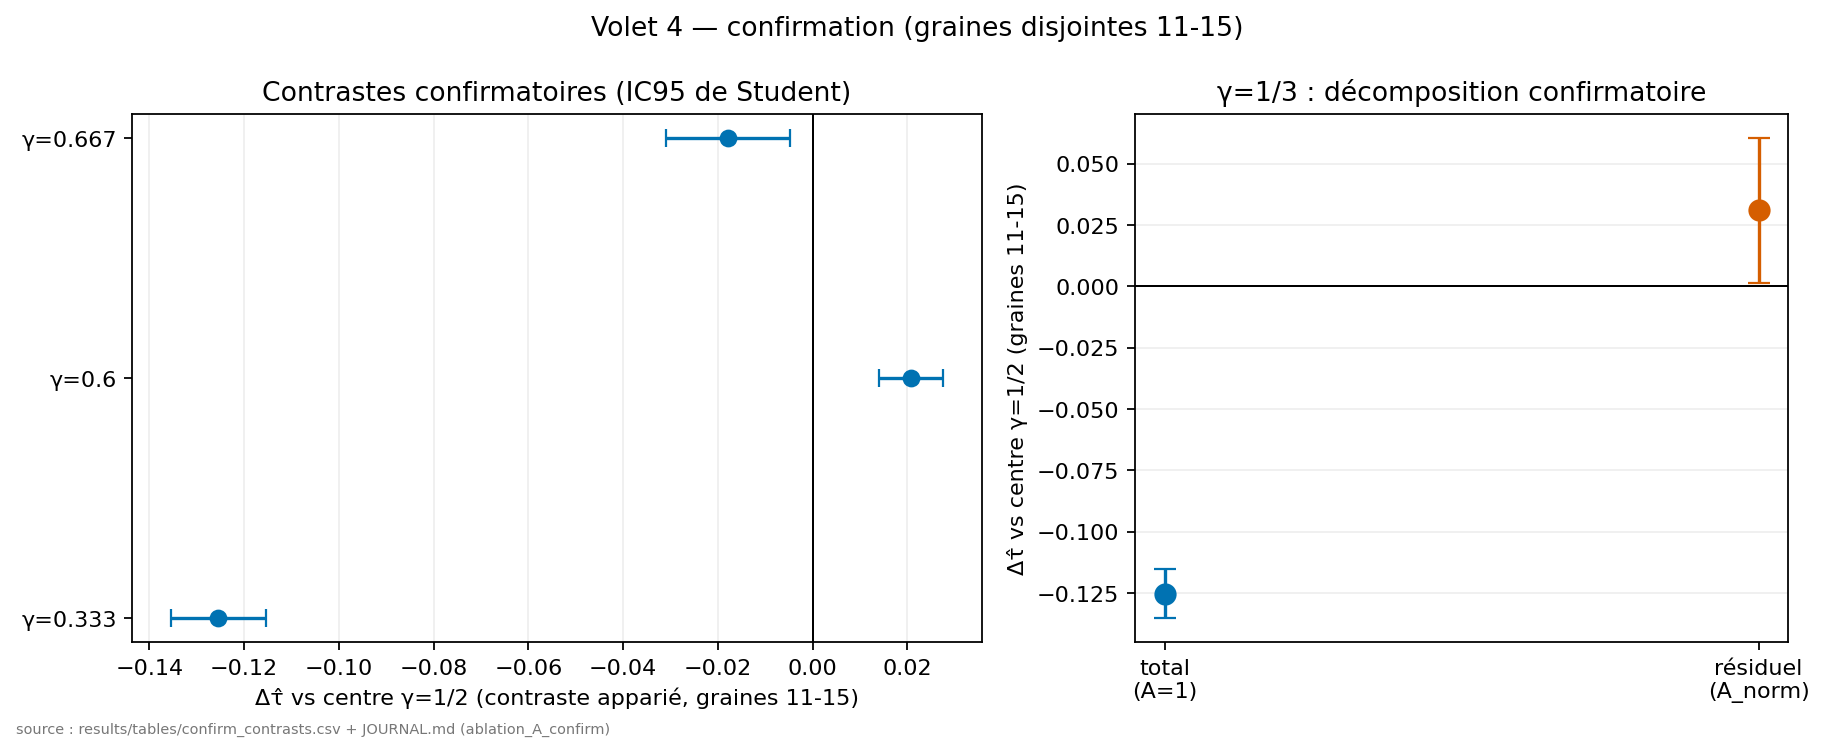
\includegraphics[width=.95\textwidth]{confirm_forest.png}
\end{center}

\begin{center}
\begin{tabular}{lrrl}
\toprule
Contraste & $\Delta\hat\tau$ & IC95 & Conditions PASS / FAIL / N\textbackslash A\\
\midrule
$\gamma=1/3$ vs $1/2$ & $-0{,}125$ & $[-0{,}135;-0{,}115]$ & 1,2,3,4,6,7 / 5,8 / --\\
$\gamma=0{,}6$ vs $1/2$ & $+0{,}021$ & $[+0{,}014;+0{,}028]$ & 1,2,6 / 4,5,7,8 / 3\\
$\gamma=2/3$ vs $1/2$ & $-0{,}018$ & $[-0{,}031;-0{,}005]$ & 1,3,6 / 2,4,5,7 / --\\
\bottomrule
\end{tabular}
\end{center}

\textbf{Erratum méthodologique (condition 5, transparence complète)} :
le test de Vuong disponible (\code{vuong\_pl\_vs\_ln}) compare la loi
\emph{pure} au log-normal. Or la loi pure est rejetée par LRT dans
\emph{les 20 runs confirmatoires} ($p<4\cdot10^{-33}$ partout, comme dans
la campagne M4B). Ce Vuong échoue donc identiquement en cellule et en
centre ($z=-5{,}5$ à $-7{,}2$, 20/20 runs) : c'est un artefact
d'outillage non différentiel, pas une preuve contre un contraste
spécifique. Diagnostic correctif : un test de Vuong \emph{correctement
normalisé} comparant la tronquée (modèle primaire) au log-normal, sur le
même support fini, donne $z=+16$ à $+19$ dans tous les runs
confirmatoires --- la famille primaire est massivement défendable. La
condition 5 est rapportée FAIL au sens littéral du protocole
(transparence), avec ce correctif documenté ; le code de décision n'a
pas été modifié rétroactivement.

\textbf{Verdict} : le contraste $\gamma=1/3$ est le seul qui satisfasse
la majorité des conditions de robustesse (IC apparié, persistance en
taille, fenêtres/horizon, scan de $s_{\min}$, stationnarité, quadrature) —
il échoue la condition 8, ce qui est en réalité l'information la plus
importante (\S\ref{sec:ablation}). Les contrastes $\gamma=0{,}6$ et
$2/3$ sont statistiquement significatifs par l'IC apparié seul mais ne
survivent pas à la robustesse complète (persistance en taille incertaine
ou nulle, quadrature défaillante) : le \og pic \fg{} vu en exploration à
$\gamma=0{,}6$ n'est pas confirmé comme un effet robuste et distinct du
bruit.

\section{Contrôle d'échelle apparié}
\label{sec:ablation}

\begin{center}
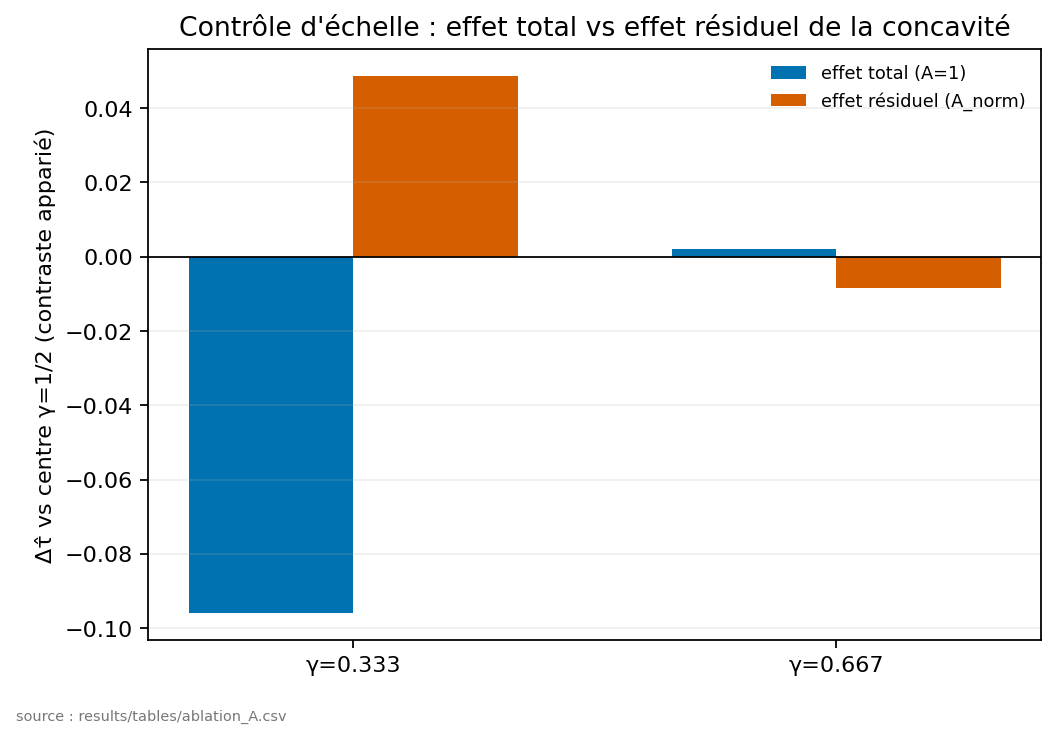
\includegraphics[width=.85\textwidth]{ablation_scale.png}
\end{center}

Décomposition effet total ($A=1$) vs effet résiduel
($A_{\mathrm{norm}}(\gamma)=19^{1-2\gamma}$, $K_{\mathrm{ref}}=361$ J),
contrastes appariés par graine (\code{results/tables/ablation\_A.csv}) :

\begin{center}
\begin{tabular}{lrrrl}
\toprule
$\gamma$ & Total ($A{=}1$) & Résiduel ($A_{\mathrm{norm}}$) & Part d'échelle & Graines\\
\midrule
$1/3$ (exploration) & $-0{,}096$ & $+0{,}049$ & $-0{,}145$ & 1--3\\
$1/3$ (\textbf{confirmatoire}) & $-0{,}125$ & $\mathbf{+0{,}031}$ & $-0{,}156$ & 11--15\\
$0{,}6$ (exploration) & $+0{,}038$ & $-0{,}006$ & $+0{,}044$ & 1--3\\
$2/3$ (exploration) & $+0{,}002$ & $-0{,}008$ & $+0{,}010$ & 1--3\\
\bottomrule
\end{tabular}
\end{center}

\textbf{Résultat robuste sur graines disjointes, significativité
marginale pour le résidu} : à échelle autarcique égalisée
($K_{\mathrm{ref}}=361$ J pour $\gamma=1/3$ et $\gamma=1/2$), l'effet
résiduel de la courbure vaut $+0{,}031$ (IC95 $[+0{,}001;+0{,}061]$,
$n=5$, graines 11--15, borne basse à $0{,}0014$, $p\approx0{,}05$) ---
de \textbf{signe opposé} à l'effet total ($-0{,}125$) et d'amplitude
quatre fois plus petite. Ce renversement de signe (le fait scientifique
robuste, indépendant de la significativité marginale du résidu lui-même)
est reproduit sur les trois contrastes ($\gamma=1/3$, $0{,}6$, $2/3$) et
sur graines confirmatoires disjointes des graines d'exploration pour
$\gamma=1/3$ : ce n'est pas un artefact de graine.

\textbf{Conclusion (condition 8 du protocole, qui échoue à bon droit)} :
l'effet mesuré de $\gamma$ sur $\hat\tau$ à $A=1$ n'est \emph{pas}
principalement un effet de concavité. Il est dominé par le déplacement
du point fixe autarcique $\Kaut(\gamma)$, qui fait varier le rapport
adimensionnel $K_0/\Kaut(\gamma,A)$ de près de deux décades le long de la
grille (de $0{,}301$ à $\gamma=1/3$ jusqu'à $3{,}645\cdot10^{-3}$ à
$\gamma=2/3$). C'est exactement la nature de confusion que le prompt de
recherche demandait explicitement de démêler (\og un changement
d'échelle du capital \fg). Ce n'est pas qu'une observation empirique :
\code{spec\_m4\_2.pdf} §7 démontre que la transformation
$(K,K_0,A)\mapsto(cK,cK_0,c^{1-\gamma}A)$ laisse exactement invariante
toute l'histoire discrète du modèle, ce qui implique nécessairement
qu'à $\gamma$ fixé $\hat\tau$ ne peut dépendre de $A,K_0$ qu'à travers
$K_0/\Kaut(\gamma,A)$.

\section{Volet mécanisme et hypothèse structurelle}
\label{sec:mecanisme}

\subsection{Chaîne causale (instantanés denses, graine 1)}

\begin{center}
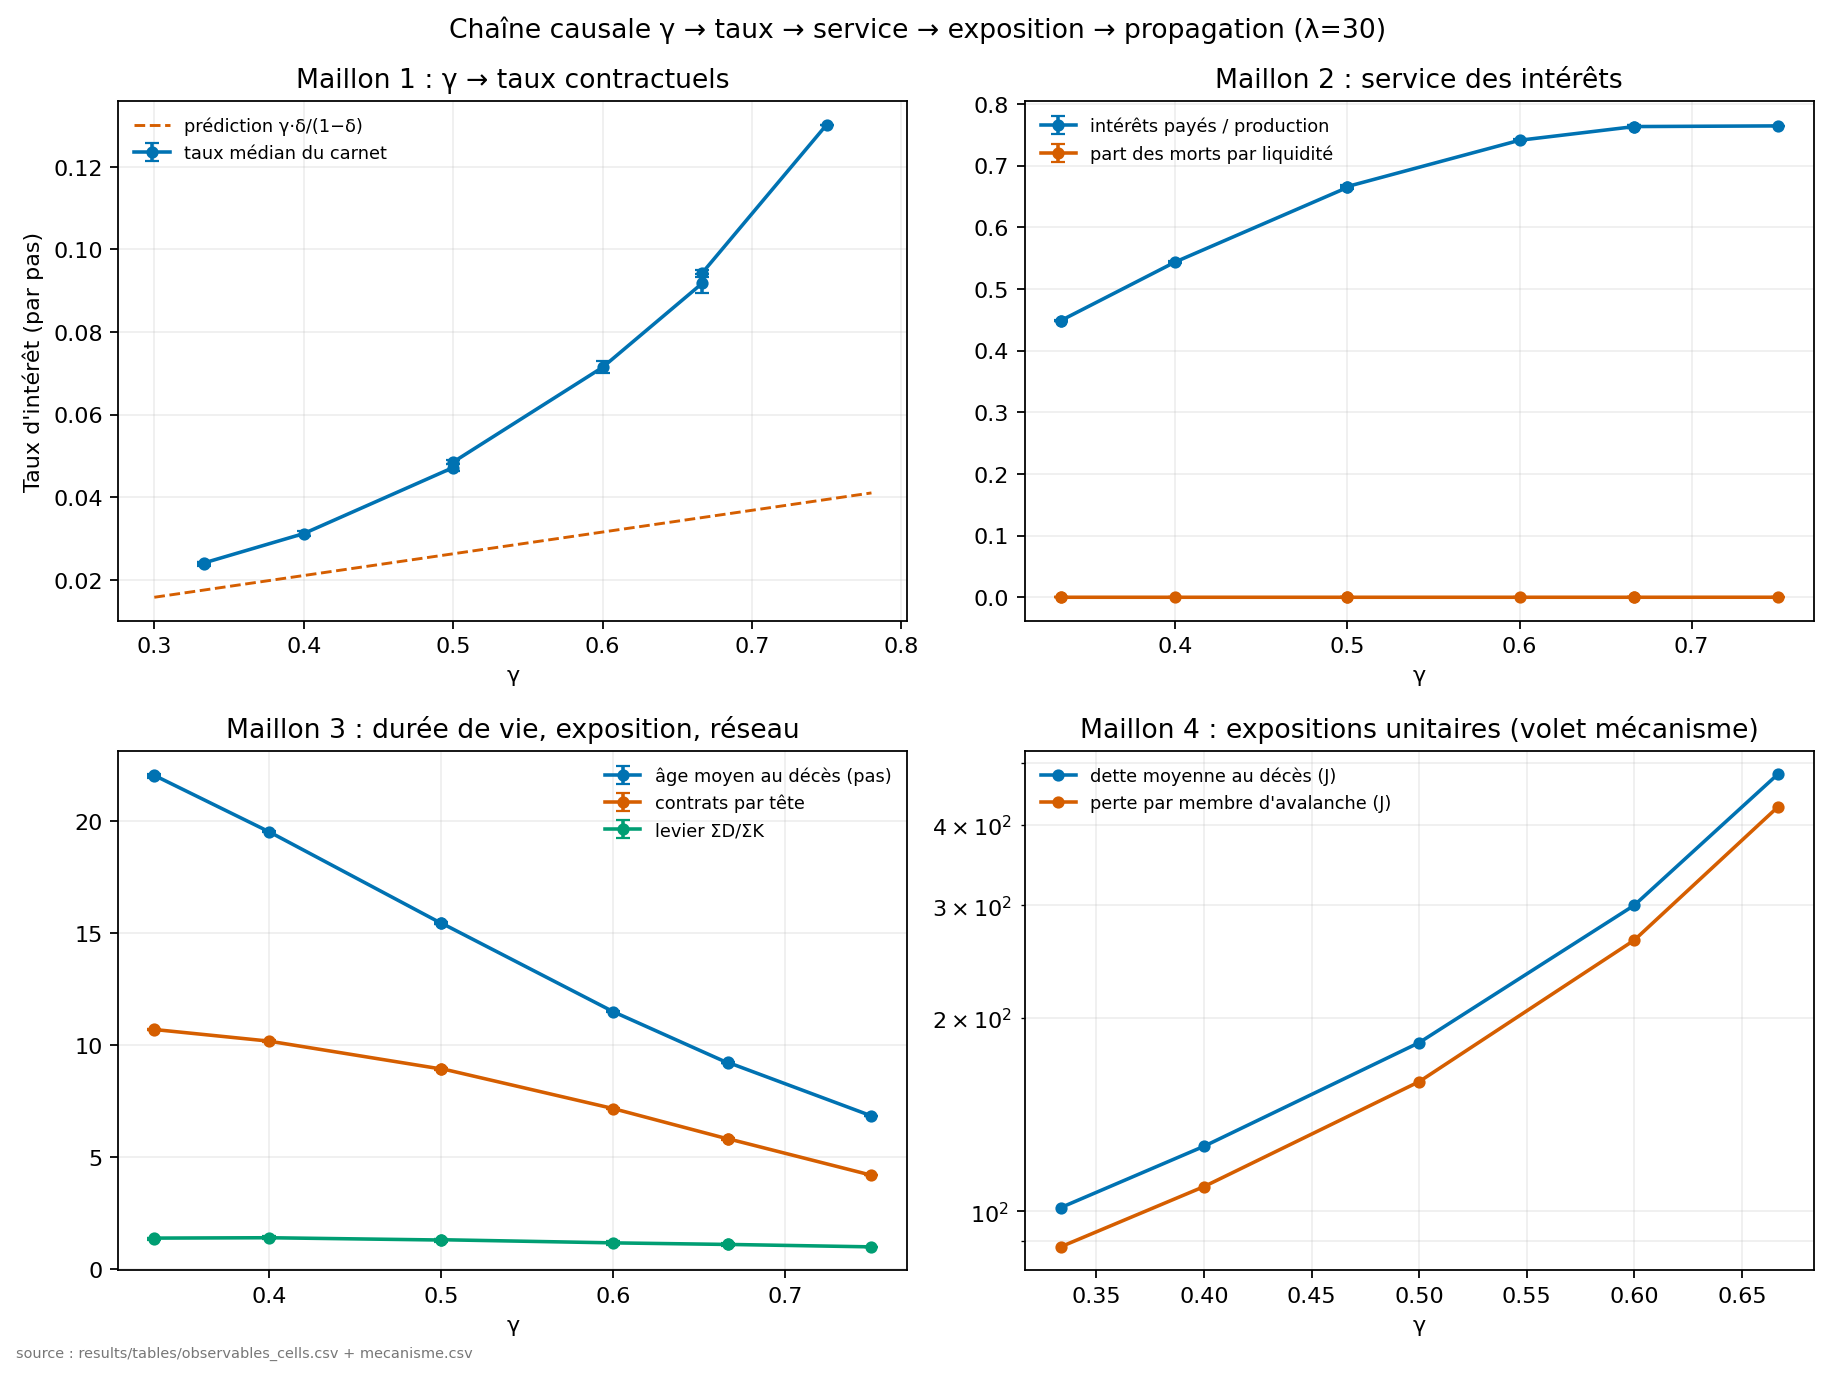
\includegraphics[width=.95\textwidth]{mechanism_chain.png}
\end{center}

Les quatre maillons proposés par le cahier des charges sont quantifiés
(\code{results/tables/mecanisme.csv}) : $\gamma$ élève le taux médian du
carnet (maillon 1, de $1{,}4$ à $2{,}7\times$ la prédiction autarcique
$\gamma\delta/(1-\delta)$, croissant avec $\gamma$ --- les contrats se
signent entre entités dont le capital reste bien en-dessous de $\Kaut$) ;
alourdit le service relatif et raccourcit les vies (maillon 2--3, âge
moyen au décès $22{,}0\to6{,}8$ pas) ; amincit le réseau (contrats par
tête $10{,}7\to4{,}2$, levier $\Sigma D/\Sigma K$ $1{,}39\to0{,}98$) ; et
la dette moyenne au décès comme la perte moyenne par membre d'avalanche
croissent d'un facteur $\approx5$ (maillon 4, $\approx100\to400$ J).
\textbf{Défaut de service quasi absent, concentré à $\gamma$ élevé} :
$17$ événements distincts sur $102$ runs, exclusivement à
$\gamma\in\{2/3,0{,}75\}$ --- jamais à $\gamma\le0{,}6$, jamais en
confirmation. La propagation reste très majoritairement une contagion de
bilan pure, comme dans M4B à $\sigma=0{,}25$, mais le canal de liquidité
s'y éveille faiblement à grand $\gamma$, cohérent avec l'alourdissement
mesuré du service (maillon 2).

\subsection{Hypothèse structurelle : $K_0/\Kaut(\gamma,A)$}

L'invariance d'échelle exacte démontrée (\code{spec\_m4\_2.pdf} §7)
établit, comme théorème et non comme hypothèse, que la cible instantanée
$\sqrt{K_\ell K_b}$ ne dépend jamais de $\gamma$ à capitaux donnés, et
qu'à $\gamma$ fixé $\hat\tau$ ne peut dépendre de $A,K_0$ qu'à travers le
rapport adimensionnel $K_0/\Kaut(\gamma,A)$. Faire varier $\gamma$ à
$A=1$ fait dériver ce rapport de $0{,}301$ ($\gamma=1/3$) à
$3{,}645\cdot10^{-3}$ ($\gamma=2/3$), soit près de deux décades. Reste à
tester la partie empirique : \emph{à ce rapport fixé, la courbure a-t-elle
encore un effet propre ?}

\textbf{Test ciblé, exploratoire} (plan \code{hypothese\_K0}, 3 graines,
$\gamma=1/2$ fixé, $A=1$, seul $K_0$ varié pour reproduire les rapports
extrêmes de la grille $\gamma$ ; contrastes appariés par graine, pas
comparaison des écarts-types de cellule) :
\begin{center}
\begin{tabular}{lrrl}
\toprule
Contraste (graines appariées, $n=3$) & $\Delta\hat\tau$ & IC95 & \\
\midrule
$\gamma=1/3$ réel $-$ $K_0$-substitution (ratio $0{,}301$) & $+0{,}001$ & $[-0{,}096;+0{,}098]$ & IC95 $\ni0$\\
$\gamma=2/3$ réel $-$ $K_0$-substitution (ratio $0{,}00364$) & $-0{,}050$ & $[-0{,}114;+0{,}014]$ & IC95 $\ni0$\\
\bottomrule
\end{tabular}
\end{center}

\textbf{À la précision disponible (3 graines), les deux contrastes sont
statistiquement indiscernables de zéro} : la demi-largeur de l'IC
apparié ($\approx0{,}1$) est du même ordre que l'effet total à expliquer
($-0{,}125$). Le test corrobore la partie \emph{nécessaire} de
l'hypothèse (le rapport $K_0/\Kaut$ est, par construction du modèle, le
seul canal possible pour $A$ et $K_0$) mais ne permet \textbf{ni
d'établir ni d'exclure} un résidu de courbure propre à $\gamma$ fixé ---
un panel de graines plus large serait nécessaire pour trancher ce point,
laissé pour une extension future.

\section{Résultats négatifs et limites}

\begin{itemize}
\item Aucune cellule éteinte, divergente, censurée ou instable sur
102 runs distincts (117 exécutions de cellule, 15 partagées entre
pilotes et taille finie) ; aucun marché inactif (taux de succès des tentatives
$\approx1$, fusions $\approx2\,\%$).
\item \textbf{L'effet de $\gamma$ sur $\hat\tau$ n'est pas un effet de
concavité} : c'est le résultat négatif central de la campagne, établi
avec la même rigueur confirmatoire que l'effet lui-même
(\S\ref{sec:ablation}). Une lecture naïve du contraste total aurait
conclu à tort que $\gamma$ \og pilote la pente \fg{} par la courbure.
\item Les contrastes $\gamma=0{,}6$ et $\gamma=2/3$, significatifs en
exploration, \textbf{ne survivent pas} à la robustesse complète en
confirmation (persistance en taille marginale ou nulle, quadrature
défaillante) : la relation $\hat\tau(\gamma)$ n'est confirmée de façon
robuste qu'au flanc bas de la grille ($\gamma\le1/2$).
\item Condition de confirmation n°5 (famille défendable) : échec
littéral universel et non différentiel dû à un choix d'outillage
(Vuong pure/log-normale au lieu de tronquée/log-normale) --- documenté
et corrigé par un diagnostic additif sans modification rétroactive du
critère (\S\ref{sec:confirm}).
\item À $\lambda=100$, $T=4000$, la coupure est systématiquement hors
portée : $\hat s_c$ n'est pas identifiable à cette taille (hérité de
M4B) ; les scalings de coupure reposent sur $\lambda\in\{10,30\}$
(2 points, indicatif).
\item Fenêtres $T/8$--$T/2$ emboîtées : contrôle faible par
construction ; la robustesse s'appuie sur l'horizon doublé, qui confirme
le contraste principal.
\item La sonde $\gamma=0{,}75$ n'a qu'une graine (jamais confirmatoire) ;
le test de l'hypothèse structurelle ($K_0$) n'a que 3 graines
d'exploration, non répété en confirmation (budget).
\end{itemize}

% Annexe générée par scripts/make_annexe.py — ne pas éditer à la main.
\section*{Annexe : traçabilité des simulations}
Chaque run est un run Simulation Lab (dossier \code{simulation\_lab\_data/runs/<run\_id>}) ; la correspondance cellule $\to$ runs est dans \code{manifests/*.manifest.json}. Les fits par run sont dans \code{results/metrics/<run\_id>.json} et les agrégats dans \code{results/tables/}.
\begin{small}
\begin{longtable}{llllrrrl}
\toprule
run\_id & plan & cellule & graine & $\gamma$ & $\lambda$ & $T$ & statut\\
\midrule
\endhead
\code{20260727\_160954\_29051328} & benchmark & bench\_g067 & 1 & 0.667 & 30 & 4000 & completed\\
\code{20260727\_160954\_d7c9806c} & benchmark & bench\_g033 & 1 & 0.333 & 30 & 4000 & completed\\
\code{20260727\_161533\_9b2ab740} & pilotes & g040 & 1 & 0.400 & 30 & 4000 & completed\\
\code{20260727\_161533\_dfa5f765} & pilotes & g040 & 2 & 0.400 & 30 & 4000 & completed\\
\code{20260727\_161533\_7ccc4ceb} & pilotes & g040 & 3 & 0.400 & 30 & 4000 & completed\\
\code{20260727\_161533\_be4cd8c8} & pilotes & g033 & 1 & 0.333 & 30 & 4000 & completed\\
\code{20260727\_161533\_128eec20} & pilotes & g033 & 2 & 0.333 & 30 & 4000 & completed\\
\code{20260727\_161533\_986a783a} & pilotes & g033 & 3 & 0.333 & 30 & 4000 & completed\\
\code{20260727\_162133\_2a12e894} & pilotes & g060 & 1 & 0.600 & 30 & 4000 & completed\\
\code{20260727\_162133\_bed8a893} & pilotes & g060 & 2 & 0.600 & 30 & 4000 & completed\\
\code{20260727\_162133\_73b818c9} & pilotes & g060 & 3 & 0.600 & 30 & 4000 & completed\\
\code{20260727\_162110\_0f51704c} & pilotes & g050 & 1 & 0.500 & 30 & 4000 & completed\\
\code{20260727\_162110\_7bedce89} & pilotes & g050 & 2 & 0.500 & 30 & 4000 & completed\\
\code{20260727\_162110\_9eee0426} & pilotes & g050 & 3 & 0.500 & 30 & 4000 & completed\\
\code{20260727\_162603\_57b6df9a} & pilotes & g075\_sonde & 1 & 0.750 & 30 & 4000 & completed\\
\code{20260727\_162531\_d36bad55} & pilotes & g067 & 1 & 0.667 & 30 & 4000 & completed\\
\code{20260727\_162531\_04dfd5f8} & pilotes & g067 & 2 & 0.667 & 30 & 4000 & completed\\
\code{20260727\_162531\_09d69b7e} & pilotes & g067 & 3 & 0.667 & 30 & 4000 & completed\\
\code{20260727\_161533\_be4cd8c8} & taille\_finie & g033 & 1 & 0.333 & 30 & 4000 & completed\\
\code{20260727\_161533\_128eec20} & taille\_finie & g033 & 2 & 0.333 & 30 & 4000 & completed\\
\code{20260727\_161533\_986a783a} & taille\_finie & g033 & 3 & 0.333 & 30 & 4000 & completed\\
\code{20260727\_163104\_a1225eb5} & taille\_finie & g033\_lam10 & 1 & 0.333 & 10 & 8000 & completed\\
\code{20260727\_163104\_b0236ff4} & taille\_finie & g033\_lam10 & 2 & 0.333 & 10 & 8000 & completed\\
\code{20260727\_163104\_fedefddd} & taille\_finie & g033\_lam10 & 3 & 0.333 & 10 & 8000 & completed\\
\code{20260727\_163555\_e4f8c832} & taille\_finie & g040\_lam10 & 1 & 0.400 & 10 & 8000 & completed\\
\code{20260727\_163555\_98e76c0a} & taille\_finie & g040\_lam10 & 2 & 0.400 & 10 & 8000 & completed\\
\code{20260727\_163555\_c70f3ee7} & taille\_finie & g040\_lam10 & 3 & 0.400 & 10 & 8000 & completed\\
\code{20260727\_161533\_9b2ab740} & taille\_finie & g040 & 1 & 0.400 & 30 & 4000 & completed\\
\code{20260727\_161533\_dfa5f765} & taille\_finie & g040 & 2 & 0.400 & 30 & 4000 & completed\\
\code{20260727\_161533\_7ccc4ceb} & taille\_finie & g040 & 3 & 0.400 & 30 & 4000 & completed\\
\code{20260727\_163104\_bef132ad} & taille\_finie & g033\_lam100 & 1 & 0.333 & 100 & 4000 & completed\\
\code{20260727\_163104\_4b9ce8fe} & taille\_finie & g033\_lam100 & 2 & 0.333 & 100 & 4000 & completed\\
\code{20260727\_163104\_68bd7116} & taille\_finie & g033\_lam100 & 3 & 0.333 & 100 & 4000 & completed\\
\code{20260727\_165050\_35fb9cc5} & taille\_finie & g050\_lam10 & 1 & 0.500 & 10 & 8000 & completed\\
\code{20260727\_165050\_00887418} & taille\_finie & g050\_lam10 & 2 & 0.500 & 10 & 8000 & completed\\
\code{20260727\_165050\_c34d4c25} & taille\_finie & g050\_lam10 & 3 & 0.500 & 10 & 8000 & completed\\
\code{20260727\_162110\_0f51704c} & taille\_finie & g050 & 1 & 0.500 & 30 & 4000 & completed\\
\code{20260727\_162110\_7bedce89} & taille\_finie & g050 & 2 & 0.500 & 30 & 4000 & completed\\
\code{20260727\_162110\_9eee0426} & taille\_finie & g050 & 3 & 0.500 & 30 & 4000 & completed\\
\code{20260727\_164035\_9df38b9c} & taille\_finie & g040\_lam100 & 1 & 0.400 & 100 & 4000 & completed\\
\code{20260727\_164035\_c77fba58} & taille\_finie & g040\_lam100 & 2 & 0.400 & 100 & 4000 & completed\\
\code{20260727\_164035\_f8cfdf9a} & taille\_finie & g040\_lam100 & 3 & 0.400 & 100 & 4000 & completed\\
\code{20260727\_165854\_e9868cc7} & taille\_finie & g060\_lam10 & 1 & 0.600 & 10 & 8000 & completed\\
\code{20260727\_165854\_1ed8e88b} & taille\_finie & g060\_lam10 & 2 & 0.600 & 10 & 8000 & completed\\
\code{20260727\_165854\_ad44077d} & taille\_finie & g060\_lam10 & 3 & 0.600 & 10 & 8000 & completed\\
\code{20260727\_162133\_2a12e894} & taille\_finie & g060 & 1 & 0.600 & 30 & 4000 & completed\\
\code{20260727\_162133\_bed8a893} & taille\_finie & g060 & 2 & 0.600 & 30 & 4000 & completed\\
\code{20260727\_162133\_73b818c9} & taille\_finie & g060 & 3 & 0.600 & 30 & 4000 & completed\\
\code{20260727\_165510\_efa1748f} & taille\_finie & g050\_lam100 & 1 & 0.500 & 100 & 4000 & completed\\
\code{20260727\_165510\_1a2ac6e9} & taille\_finie & g050\_lam100 & 2 & 0.500 & 100 & 4000 & completed\\
\code{20260727\_165510\_7cfb5d17} & taille\_finie & g050\_lam100 & 3 & 0.500 & 100 & 4000 & completed\\
\code{20260727\_171108\_35986207} & taille\_finie & g067\_lam10 & 1 & 0.667 & 10 & 8000 & completed\\
\code{20260727\_171108\_1ccc839e} & taille\_finie & g067\_lam10 & 2 & 0.667 & 10 & 8000 & completed\\
\code{20260727\_171108\_708b7b8f} & taille\_finie & g067\_lam10 & 3 & 0.667 & 10 & 8000 & completed\\
\code{20260727\_162531\_d36bad55} & taille\_finie & g067 & 1 & 0.667 & 30 & 4000 & completed\\
\code{20260727\_162531\_04dfd5f8} & taille\_finie & g067 & 2 & 0.667 & 30 & 4000 & completed\\
\code{20260727\_162531\_09d69b7e} & taille\_finie & g067 & 3 & 0.667 & 30 & 4000 & completed\\
\code{20260727\_170313\_45bf4b8f} & taille\_finie & g060\_lam100 & 1 & 0.600 & 100 & 4000 & completed\\
\code{20260727\_170313\_a4a2f4fa} & taille\_finie & g060\_lam100 & 2 & 0.600 & 100 & 4000 & completed\\
\code{20260727\_170313\_f3ec93f2} & taille\_finie & g060\_lam100 & 3 & 0.600 & 100 & 4000 & completed\\
\code{20260727\_171520\_cab04bf8} & taille\_finie & g067\_lam100 & 1 & 0.667 & 100 & 4000 & completed\\
\code{20260727\_171520\_3e7f3be9} & taille\_finie & g067\_lam100 & 2 & 0.667 & 100 & 4000 & completed\\
\code{20260727\_171520\_790e6788} & taille\_finie & g067\_lam100 & 3 & 0.667 & 100 & 4000 & completed\\
\code{20260727\_172713\_c3eaf564} & horizon\_double & g050\_T8000 & 1 & 0.500 & 30 & 8000 & completed\\
\code{20260727\_172713\_8822ea62} & horizon\_double & g050\_T8000 & 2 & 0.500 & 30 & 8000 & completed\\
\code{20260727\_172713\_eca29fdc} & horizon\_double & g050\_T8000 & 3 & 0.500 & 30 & 8000 & completed\\
\code{20260727\_172713\_f6b48923} & horizon\_double & g033\_T8000 & 1 & 0.333 & 30 & 8000 & completed\\
\code{20260727\_172713\_2e2f81ed} & horizon\_double & g033\_T8000 & 2 & 0.333 & 30 & 8000 & completed\\
\code{20260727\_172713\_eb823f56} & horizon\_double & g033\_T8000 & 3 & 0.333 & 30 & 8000 & completed\\
\code{20260727\_174005\_b2c277c8} & horizon\_double & g067\_T8000 & 1 & 0.667 & 30 & 8000 & completed\\
\code{20260727\_174005\_4a0fab1a} & horizon\_double & g067\_T8000 & 2 & 0.667 & 30 & 8000 & completed\\
\code{20260727\_174005\_a7d2ba66} & horizon\_double & g067\_T8000 & 3 & 0.667 & 30 & 8000 & completed\\
\code{20260727\_175504\_85dee157} & confirm & g033\_confirm & 11 & 0.333 & 30 & 4000 & completed\\
\code{20260727\_175504\_da86412e} & confirm & g033\_confirm & 12 & 0.333 & 30 & 4000 & completed\\
\code{20260727\_175504\_5bc07338} & confirm & g033\_confirm & 13 & 0.333 & 30 & 4000 & completed\\
\code{20260727\_175504\_a6f95655} & confirm & g033\_confirm & 14 & 0.333 & 30 & 4000 & completed\\
\code{20260727\_175504\_05396f59} & confirm & g033\_confirm & 15 & 0.333 & 30 & 4000 & completed\\
\code{20260727\_180556\_fc9cc56c} & confirm & g050\_confirm & 11 & 0.500 & 30 & 4000 & completed\\
\code{20260727\_180556\_3b538fea} & confirm & g050\_confirm & 12 & 0.500 & 30 & 4000 & completed\\
\code{20260727\_180556\_ffc1e03b} & confirm & g050\_confirm & 13 & 0.500 & 30 & 4000 & completed\\
\code{20260727\_180556\_bed0e50b} & confirm & g050\_confirm & 14 & 0.500 & 30 & 4000 & completed\\
\code{20260727\_180556\_d0c58064} & confirm & g050\_confirm & 15 & 0.500 & 30 & 4000 & completed\\
\code{20260727\_181536\_0fb74787} & confirm & g060\_confirm & 11 & 0.600 & 30 & 4000 & completed\\
\code{20260727\_181536\_0f37e2cb} & confirm & g060\_confirm & 12 & 0.600 & 30 & 4000 & completed\\
\code{20260727\_181536\_14a294b8} & confirm & g060\_confirm & 13 & 0.600 & 30 & 4000 & completed\\
\code{20260727\_181536\_aa4e0c09} & confirm & g060\_confirm & 14 & 0.600 & 30 & 4000 & completed\\
\code{20260727\_181536\_d787f683} & confirm & g060\_confirm & 15 & 0.600 & 30 & 4000 & completed\\
\code{20260727\_182401\_5542d4b4} & confirm & g067\_confirm & 11 & 0.667 & 30 & 4000 & completed\\
\code{20260727\_182402\_8574a621} & confirm & g067\_confirm & 12 & 0.667 & 30 & 4000 & completed\\
\code{20260727\_182402\_dcc5afba} & confirm & g067\_confirm & 13 & 0.667 & 30 & 4000 & completed\\
\code{20260727\_182402\_1c5fe2b8} & confirm & g067\_confirm & 14 & 0.667 & 30 & 4000 & completed\\
\code{20260727\_182402\_2b851ed1} & confirm & g067\_confirm & 15 & 0.667 & 30 & 4000 & completed\\
\code{20260727\_183204\_0c234778} & ablation\_A & g060\_Anorm & 1 & 0.600 & 30 & 4000 & completed\\
\code{20260727\_183204\_7fea484e} & ablation\_A & g060\_Anorm & 2 & 0.600 & 30 & 4000 & completed\\
\code{20260727\_183204\_0bc048a2} & ablation\_A & g060\_Anorm & 3 & 0.600 & 30 & 4000 & completed\\
\code{20260727\_183204\_b7c8fd58} & ablation\_A & g033\_Anorm & 1 & 0.333 & 30 & 4000 & completed\\
\code{20260727\_183204\_bbb241d1} & ablation\_A & g033\_Anorm & 2 & 0.333 & 30 & 4000 & completed\\
\code{20260727\_183204\_13506a8c} & ablation\_A & g033\_Anorm & 3 & 0.333 & 30 & 4000 & completed\\
\code{20260727\_183808\_16957da0} & ablation\_A & g067\_Anorm & 1 & 0.667 & 30 & 4000 & completed\\
\code{20260727\_183808\_f4780243} & ablation\_A & g067\_Anorm & 2 & 0.667 & 30 & 4000 & completed\\
\code{20260727\_183808\_5ebeae50} & ablation\_A & g067\_Anorm & 3 & 0.667 & 30 & 4000 & completed\\
\code{20260729\_143545\_56cf0dee} & ablation\_A\_confirm & g033\_Anorm\_confirm & 11 & 0.333 & 30 & 4000 & completed\\
\code{20260729\_143546\_0f543b0a} & ablation\_A\_confirm & g033\_Anorm\_confirm & 12 & 0.333 & 30 & 4000 & completed\\
\code{20260729\_143546\_08c4a4d0} & ablation\_A\_confirm & g033\_Anorm\_confirm & 13 & 0.333 & 30 & 4000 & completed\\
\code{20260729\_143546\_0bf46b26} & ablation\_A\_confirm & g033\_Anorm\_confirm & 14 & 0.333 & 30 & 4000 & completed\\
\code{20260729\_143546\_ccb0ded4} & ablation\_A\_confirm & g033\_Anorm\_confirm & 15 & 0.333 & 30 & 4000 & completed\\
\code{20260727\_184355\_b8b2e9f7} & mecanisme & g067\_meca & 1 & 0.667 & 30 & 4000 & completed\\
\code{20260727\_184355\_a1bca015} & mecanisme & g060\_meca & 1 & 0.600 & 30 & 4000 & completed\\
\code{20260727\_184355\_1e0896c8} & mecanisme & g050\_meca & 1 & 0.500 & 30 & 4000 & completed\\
\code{20260727\_184355\_6a568c58} & mecanisme & g040\_meca & 1 & 0.400 & 30 & 4000 & completed\\
\code{20260727\_184355\_e31165e7} & mecanisme & g033\_meca & 1 & 0.333 & 30 & 4000 & completed\\
\code{20260727\_185754\_f69d6fd3} & hypothese\_K0 & k0\_match\_g067 & 1 & 0.500 & 30 & 4000 & completed\\
\code{20260727\_185754\_873a545d} & hypothese\_K0 & k0\_match\_g067 & 2 & 0.500 & 30 & 4000 & completed\\
\code{20260727\_185754\_c39807ce} & hypothese\_K0 & k0\_match\_g067 & 3 & 0.500 & 30 & 4000 & completed\\
\code{20260727\_185754\_bb75a633} & hypothese\_K0 & k0\_match\_g033 & 1 & 0.500 & 30 & 4000 & completed\\
\code{20260727\_185754\_849aa693} & hypothese\_K0 & k0\_match\_g033 & 2 & 0.500 & 30 & 4000 & completed\\
\code{20260727\_185754\_f48f5035} & hypothese\_K0 & k0\_match\_g033 & 3 & 0.500 & 30 & 4000 & completed\\
\bottomrule
\end{longtable}
\end{small}
\noindent Total : 117 exécutions de cellule (102 runs Simulation Lab distincts ; 15 partagés entre plans par identifiant de cellule). Condensat(s) moteur : 932e58643e522d7b (version \code{m4\_2-1}). Rôles des plans : \emph{benchmark} = calibrage de coût (volet 0) ; \emph{pilotes} = exploration grille $\gamma$ (volet 1) ; \emph{taille\_finie} = taille finie $\lambda$ (volet 2) ; \emph{horizon\_double} = robustesse horizon (volet 3) ; \emph{confirm} = confirmation graines 11-15 (volet 4) ; \emph{ablation\_A} = contrôle d'échelle $A_{\mathrm{norm}}$ (volet 5, exploration) ; \emph{ablation\_A\_confirm} = contrôle d'échelle $A_{\mathrm{norm}}$, graines 11-15 (volet 5 étendu) ; \emph{mecanisme} = chaîne causale (volet 6) ; \emph{hypothese\_K0} = hypothèse structurelle $K_0/K^*_{\mathrm{aut}}$ (test ciblé).

\end{document}
